\documentclass[14pt,a4paper,report]{report}
\usepackage[a4paper, mag=1000, left=2.5cm, right=1cm, top=2cm, bottom=2cm, headsep=0.7cm, footskip=1cm]{geometry}
\usepackage[utf8]{inputenc}
\usepackage[english,russian]{babel}
\usepackage{indentfirst}
\usepackage[dvipsnames]{xcolor}
\usepackage[colorlinks]{hyperref}
\usepackage{listings} 
\usepackage{fancyhdr}
\usepackage{caption}
\usepackage{graphicx}
\hypersetup{
	colorlinks = true,
	linkcolor  = black
}

\usepackage{titlesec}
\titleformat{\chapter}
{\Large\bfseries} % format
{}                % label
{0pt}             % sep
{\huge}           % before-code


\DeclareCaptionFont{white}{\color{white}} 

% Listing description
\usepackage{listings} 
\DeclareCaptionFormat{listing}{\colorbox{gray}{\parbox{\textwidth}{#1#2#3}}}
\captionsetup[lstlisting]{format=listing,labelfont=white,textfont=white}
\lstset{ 
	% Listing settings
	inputencoding = utf8,			
	extendedchars = \true, 
	keepspaces = true, 			  	 % Поддержка кириллицы и пробелов в комментариях
	language = bash,            	 	 % Язык программирования (для подсветки)
	basicstyle = \small\sffamily, 	 % Размер и начертание шрифта для подсветки кода
	numbers = left,               	 % Где поставить нумерацию строк (слева\справа)
	numberstyle = \tiny,          	 % Размер шрифта для номеров строк
	stepnumber = 1,               	 % Размер шага между двумя номерами строк
	numbersep = 5pt,              	 % Как далеко отстоят номера строк от подсвечиваемого кода
	backgroundcolor = \color{white}, % Цвет фона подсветки - используем \usepackage{color}
	showspaces = false,           	 % Показывать или нет пробелы специальными отступами
	showstringspaces = false,    	 % Показывать или нет пробелы в строках
	showtabs = false,           	 % Показывать или нет табуляцию в строках
	frame = single,              	 % Рисовать рамку вокруг кода
	tabsize = 2,                  	 % Размер табуляции по умолчанию равен 2 пробелам
	captionpos = t,             	 % Позиция заголовка вверху [t] или внизу [b] 
	breaklines = true,           	 % Автоматически переносить строки (да\нет)
	breakatwhitespace = false,   	 % Переносить строки только если есть пробел
	escapeinside = {\%*}{*)}      	 % Если нужно добавить комментарии в коде
}

\begin{document}

\def\contentsname{Contents}

% Titlepage
\begin{titlepage}
	\begin{center}
		\textsc{Peter the Great St.Petersburg Polytechnic University\\[5mm]
			Department of Computer Systems \& Software Engineering}
		
		\vfill
		
		\textbf{Laboratory report №3\\[3mm]
			Discipline: «Information Security»\\[3mm]
			Theme: «Metasploit»\\[41mm]
		}
	\end{center}
	
	\hfill
	\begin{minipage}{.4\textwidth}
		Made by student:\\[2mm] 
		Boyarkin N.S.\\
		Group: 13541/3\\[5mm]
		
		Lecturer:\\[2mm] 
		Bogach N.V.
	\end{minipage}
	\vfill
	\begin{center}
		Saint-Petersburg\\ \the\year\ y.
	\end{center}
\end{titlepage}

% Contents
\tableofcontents
\clearpage

\chapter{Laboratory work №3}

\section{Work purpose}

Study the MSFconsole core commands, Metasploit tools and how to use exploits to gain the access to the system

\section{Task}

\begin{enumerate}
	\item Basic concepts using documentation - auxiliary, payload, exploit, shellcode, nop, encoder.
	\item How to launch msfconsole and list available commands (help).
	\item MSFconsole core commands search (name, type, author etc. search), info, load, use.
	\item Using exploits.
	\item Database Backend Commands.
	\item Metasploit GUIs – Armitage GUI front-end for the Metasploit Framework.
	\item Metasploit GUIs – web-client GUI.
	\item VNC Scanner.
	\item SMB Login Check Scanner.
	\item Get root using vsftpd vulnerability.
	\item Get root using irc vulnerability.
	\item Armitage Hail Mary.
	\item Study three exploit source code files and explain them.
\end{enumerate}

\clearpage

\section{Work Progress}

\subsection{Introduction}

To take advantage of a system vulnerability, you often need an exploit, a small and highly specialized computer program whose only reason of being is to take advantage of a specific vulnerability and to provide access to a computer system. Exploits often deliver a payload to the target system to grant the attacker access to the system. The Metasploit Project host the worlds largest public database of qualityassured exploits.

\subsection{Basic concepts using documentation - auxiliary, payload, exploit, shellcode, nop, encoder}

The Metasploit framework is based on a modular architecture. This means that all the exploits, payloads, encoders etc. are present in the form of modules. The biggest advantage of a modular architecture is that it is easier to extend the functionality of the framework based on requirement.

\begin{itemize}
	\item \textbf{auxiliary} -- run without a session; used for discovery, port scanning, and brute forcing etc.
	\item \textbf{payload} -- the code that is executed after the control of the system has been received.
	\item \textbf{exploit} -- a code fragment that exploits a vulnerability in the software or OS to perform.
	an attack on the system.
	\item \textbf{shellcode} -- is the code that passes control to the shell.
	\item \textbf{nop} -- is an assembler instruction that does not perform any action.
	\item \textbf{encoder} --  is used to rid a payload of any characters which may cause issues with successful payload execution, such as null.
\end{itemize}

\subsection{How to launch msfconsole and list available commands (help)}

Let's run the metasploit framework by the \textbf{msfconsole} command:

\lstinputlisting{listings/1.1.log}

All available metasploit commands can be output by the \textbf{help} command:

\lstinputlisting{listings/1.2.log}

\subsection{MSFconsole core commands search (name, type, author etc. search), info, load, use}

The msfconsole includes an extensive regular-expression based search functionality. If you have a general idea of what you are looking for, you can search for it via \textbf{search}.

\begin{itemize}
	\item To search using a descriptive name, use the \textbf{name} keyword.
	\item You can use \textbf{platform} to narrow down your search to modules that affect a specific platform.
	\item Using the \textbf{type} lets you filter by module type such as auxiliary, post, exploit, etc.
	\item Searching with the \textbf{author} keyword lets you search for modules by your favourite author.
\end{itemize}

\lstinputlisting{listings/2.log}

Metasploit \textbf{info} command displays information about one or more module:

\lstinputlisting{listings/3.log}

\clearpage

Let's try to find some plugins to load them:

\lstinputlisting{listings/4.log}

Metasploit \textbf{load} command loads a framework plugin:

\lstinputlisting{listings/5.log}

Metasploit \textbf{use} command selects a module by name:

\lstinputlisting{listings/6.log}

\subsection{Using exploits}

Let's try to find a backdoor for Apache HTTP Server, that is running on remote Metasploitable 2 OS (192.168.56.101):

\lstinputlisting{listings/7.1.log}

Run the exploit to gain control of the remote system:

\lstinputlisting{listings/7.2.log}

\subsection{Database Backend Commands}

Metasploit \textbf{db\_connect} command connects to an existing database:

\lstinputlisting{listings/8.1.log}

We can confirm that Metasploit is successfully connected to the database by the db\_status command:

\lstinputlisting{listings/8.2.log}

Metasploit \textbf{hosts} command will display all the hosts stored in our current workspace:

\lstinputlisting{listings/8.3.log}

Another way to search the database is by using the \textbf{services} command:

\lstinputlisting{listings/8.4.log}

Issuing the \textbf{workspace} command from the msfconsole, will display the currently selected workspaces. Option -a used for creating new workspace. New workspace has empty host and services by default.

\lstinputlisting{listings/8.5.log}

Using the \textbf{db\_export} command all our gathered information can be saved in a XML file:

\lstinputlisting{listings/9.log}

\subsection{Metasploit GUIs – Armitage GUI front-end for the Metasploit Framework}

Armigate is open source software that organizes the hacking process for Metasploit. It can also work together with Nmap. The whole point of this program is that it gives an interface, facilitates the use of Metasploit and speeds up the hacking process.

When armitage started, all variables already filled with defaut data. If necessary, you can specify them:

\begin{figure}[h!]
	\centering
	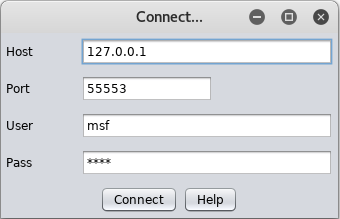
\includegraphics[scale = 1.10]{images/1.png}
	\caption{Armirage connect window}
\end{figure}

\clearpage

After that, the IP address of the remote system for hacking is specified and the main window is launched. The list of all modules is located in the left part of the window. At the bottom of the window all the commands of the metasploit console are displayed.

\begin{figure}[h!]
	\centering
	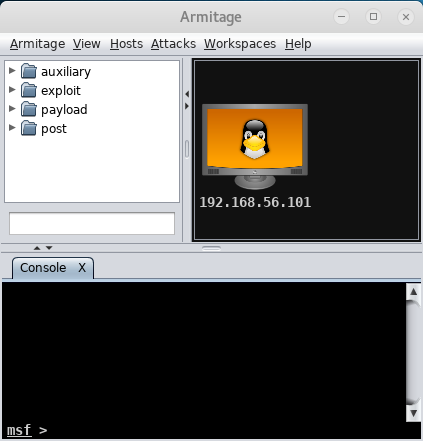
\includegraphics[scale = 0.77]{images/2.png}
	\caption{Armirage main window}
\end{figure}

The port scan is started by the utility auxiliary/scanner/portscan/tcp and can be called from the context menu:

\begin{figure}[h!]
	\centering
	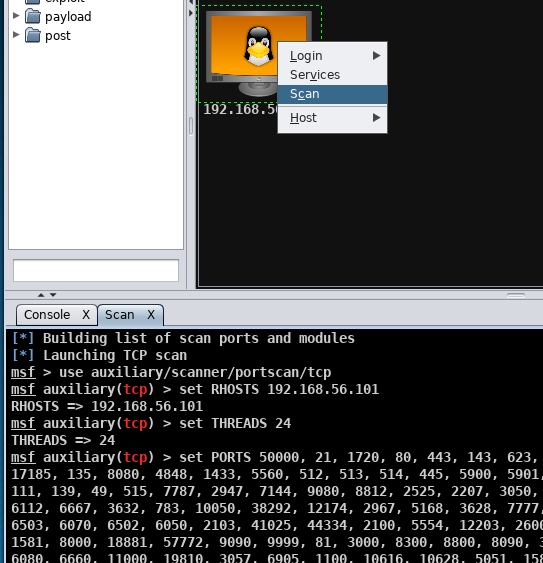
\includegraphics[scale = 0.80]{images/3.png}
	\caption{Armirage is scanning remote system}
\end{figure}

After searching for attacks in the menu Attacks -> Find Attacks, a list of possible attacks is available on each of the hosts through the context menu:

\begin{figure}[h!]
	\centering
	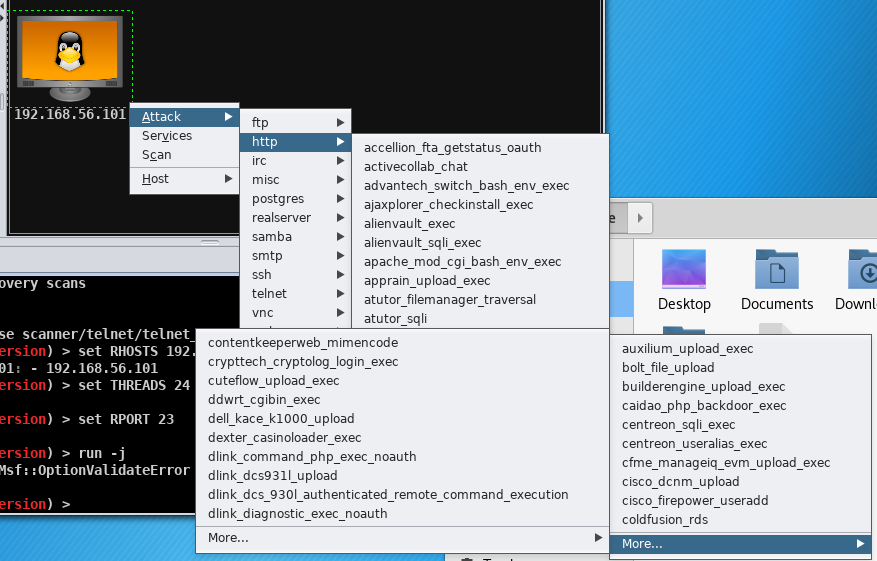
\includegraphics[scale = 0.80]{images/4.png}
	\caption{Armirage list of available attack exploits}
\end{figure}


\subsection{Metasploit GUIs – web-client GUI}

One graphical interface for Metasploit has already been considered. There is one more - \textbf{MSF Community Edition}, but it is not supported in Kali Linux.

\subsection{VNC Scanner}

The VNC server on the attacked machine (Metasploitable 2 OS) is running on port 5900:

\lstinputlisting{listings/10.log}

To scan the system for a VNC vulnerability, use the utility auxiliary/scanner/vnc/vnc\_login:

\lstinputlisting{listings/11.log}

The result was a password for VNC (password). Now we could use the \textbf{vncviewer} to connect to a remote console:

\begin{figure}[h!]
	\centering
	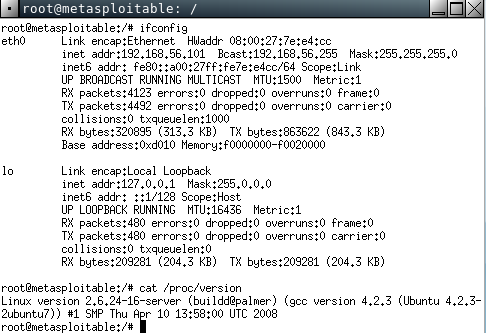
\includegraphics[scale = 0.84]{images/5.png}
	\caption{Remote console into VNCviewer}
\end{figure}

\subsection{SMB Login Check Scanner}

The smb\_enumshares module, enumerates any SMB shares that are available on a remote system:

\lstinputlisting{listings/12.log}

You can see the list of shared directories available via SMB protocol, as well as two IPC tools.

\subsection{Get root using vsftpd vulnerability}

The Metasploit Framework has an exploit available to exploit the VSFTPD v2.3.4 vulnerability. Let's tru tu run it from Armigate GUI:

\begin{figure}[h!]
	\centering
	
\includegraphics[scale = 0.90]{images/6.png}
	\caption{VSFTPD v2.3.4 exploit}
\end{figure}

At the bottom part of window we can see the command line commands:

\lstinputlisting{listings/13.log}

\clearpage

After the backdoor was successfully executed, a new shell was registered, in which commands are entered on the remote machine:

\begin{figure}[h!]
	\centering
	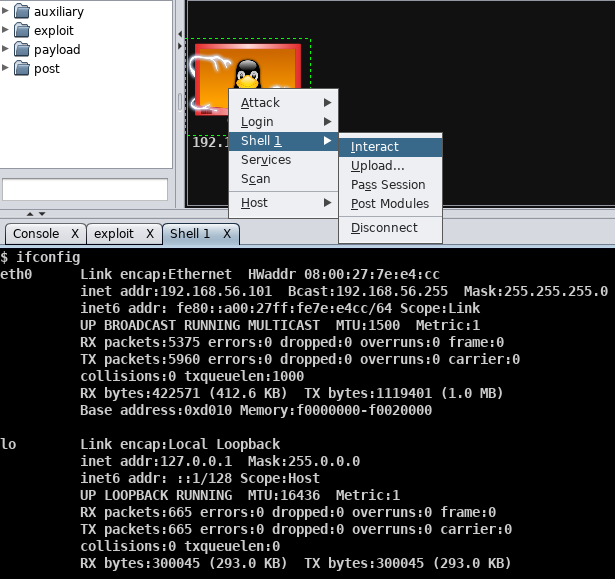
\includegraphics[scale = 0.60]{images/7.png}
	\caption{Now we have access to remote console}
\end{figure}

\subsection{Get root using IRC vulnerability}

Let's try to use exploit \textbf{/unix/irc/unreal\_ircd\_3281\_backdoor} to get remote access:

\begin{figure}[h!]
	\centering
	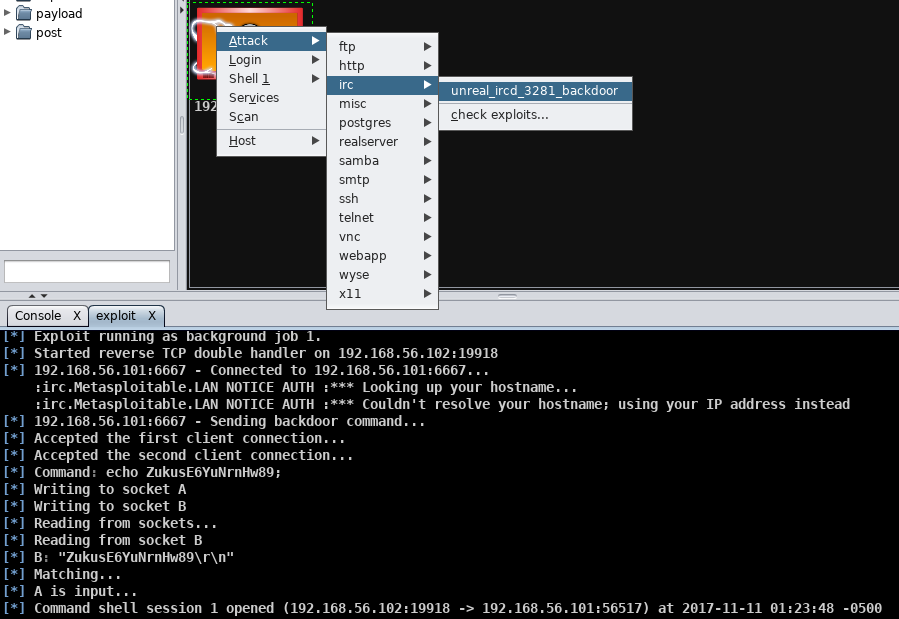
\includegraphics[scale = 0.65]{images/8.png}
	\caption{Unreal IRC exploit}
\end{figure}

After the backdoor was successfully executed, a new shell was registered, in which commands are entered on the remote machine:

\begin{figure}[h!]
	\centering
	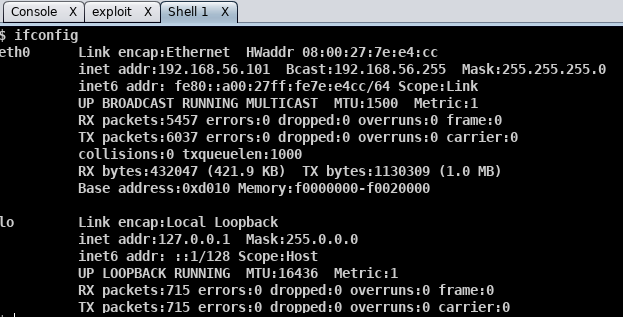
\includegraphics[scale = 0.70]{images/9.png}
	\caption{Now we have access to remote console}
\end{figure}

\subsection{Armitage Hail Mary}

Armitage recommends exploits and will optionally run active checks to tell you which exploits will work. If these options fail, use the Hail Mary attack to unleash Armitage's smart automatic exploitation against your targets.

After running the command Hail Mary, we got access to php, java, and also using 5 different exploits access to the unix shell. Information about each session, including the exploit, with which access was obtained are displayed in the console, you can connect to the session through the context menu.

\begin{figure}[h!]
	\centering
	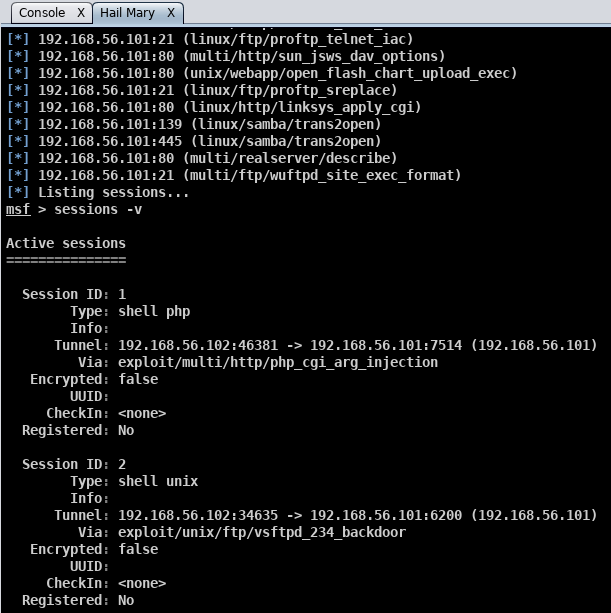
\includegraphics[scale = 0.75]{images/10.png}
	\caption{Armigate Hail Mary}
\end{figure}

\subsection{Study three exploit source code files and explain them}

Exploits source code sored at usr/share/metasploit-framework/modules/exploits directory by default. 

The source code of each exploit is divided into two parts: \textbf{initialization} and \textbf{exploit}. Initialization module contains the following information:

\begin{itemize}
	\item \textbf{Name} -- exploit name.
	\item \textbf{Description} -- the module's description.
	\item \textbf{Author} -- the array of zero or more authors.
	\item \textbf{License} -- the license under which this module is provided.
	\item \textbf{References} --  the array of zero or more references.
	\item \textbf{Platform} -- the array of zero or more platforms.
	\item \textbf{Arch} -- the array of zero or more architectures.
	\item \textbf{Privileged} -- whether or not this module requires privileged access.
	\item \textbf{Payload} -- information about payload data, which sends to the server.
	\item \textbf{Targets} -- the array of zero or more targets.
	\item \textbf{DefaultTarget} -- default target.
	\item \textbf{DisclosureDate} -- disclosure date.
\end{itemize}

The content of the exploit function differs depending on its method of operation.

\subsubsection{proftpd\_133c\_backdoor}

This backdoor exploits the vulnerability of the FTP server ProFTPd version 1.3.3c.

This script attempts to exploit the backdoor using the innocuous id command by default, but that can be changed with the ftp-proftpd-backdoor.cmd script argument.

\lstinputlisting{listings/14.rb}

\subsubsection{unreal\_ircd\_3281\_backdoor}

UnrealIRCd 3.2.8.1, as distributed on certain mirror sites from November 2009 through June 2010, contains an externally introduced modification (Trojan Horse) in the DEBUG3\_DOLOG\_SYSTEM macro, which allows remote attackers to execute arbitrary commands.

\lstinputlisting{listings/15.rb}

\subsubsection{phpmyadmin\_3522\_backdoor}

phpMyAdmin 3.5.2.2, as distributed by the cdnetworks-kr-1 mirror during an unspecified time frame in 2012, contains an externally introduced modification (Trojan Horse) in server\_sync.php, which allows remote attackers to execute arbitrary PHP code via an eval injection attack.

\lstinputlisting{listings/16.rb}

\section{Conclusion}

In this paper, tools for testing systems on various vulnerabilities have been studied. The metasploit framework greatly simplifies the process of analyzing the system on various vulnerabilities, and also allows access to various system resources using built-in exploits.

\end{document}